\documentclass[12pt]{article}
%\documentclass[12pt]{scrartcl}
%\title{ELEC 340 Assignment 3}
\nonstopmode
%\usepackage[utf8]{inputenc}
\usepackage{graphicx} % Required for including pictures
\usepackage[figurename=Figure]{caption}
\usepackage{float}    % For tables and other floats
\usepackage{verbatim} % For comments and other
\usepackage{amsmath}  % For math
%\usepackage[scr=rsfso,cal=zapfc,frak=euler,bb=ams]{mathalfa}
\usepackage{amssymb}  % For more math
\usepackage{fullpage} % Set margins and place page numbers at bottom center
\usepackage{paralist} % paragraph spacing
\usepackage{listings} % For source code
\usepackage{subfig}   % For subfigures
%\usepackage{physics}  % for simplified dv, and 
\usepackage{enumitem} % useful for itemization
\usepackage{siunitx}  % standardization of si units
\usepackage[spanish]{babel}
\usepackage[bitstream-charter,cal=cmcal]{mathdesign}
\usepackage[T1]{fontenc}
\usepackage[mathcal]{eucal}

\usepackage{tikz,bm} % Useful for drawing plots
%\usepackage{tikz-3dplot}
\usepackage{circuitikz}
\usepackage[ruled,vlined]{algorithm2e}
\usepackage{tikz}
\DeclareSymbolFont{usualmathcal}{OMS}{cmsy}{m}{n}
\DeclareSymbolFontAlphabet{\mathcal}{usualmathcal}



%%% Colours used in field vectors and propagation direction
\definecolor{mycolor}{rgb}{1,0.2,0.3}
\definecolor{brightgreen}{rgb}{0.4, 1.0, 0.0}
\definecolor{britishracinggreen}{rgb}{0.0, 0.26, 0.15}
\definecolor{cadmiumgreen}{rgb}{0.0, 0.42, 0.24}
\definecolor{ceruleanblue}{rgb}{0.16, 0.32, 0.75}
\definecolor{darkelectricblue}{rgb}{0.33, 0.41, 0.47}
\definecolor{darkpowderblue}{rgb}{0.0, 0.2, 0.6}
\definecolor{darktangerine}{rgb}{1.0, 0.66, 0.07}
\definecolor{emerald}{rgb}{0.31, 0.78, 0.47}
\definecolor{palatinatepurple}{rgb}{0.41, 0.16, 0.38}
\definecolor{pastelviolet}{rgb}{0.8, 0.6, 0.79}

\usepackage{pdfpages}
\usepackage{graphicx}
\usepackage{float}

%---------- Listings config


\usepackage{color}

\definecolor{dkgreen}{rgb}{0,0.6,0}
\definecolor{gray}{rgb}{0.5,0.5,0.5}
\definecolor{mauve}{rgb}{0.58,0,0.82}

\lstset{frame=tb,
  language=Java,
  aboveskip=3mm,
  belowskip=3mm,
  showstringspaces=false,
  columns=flexible,
  basicstyle={\small\ttfamily},
  numbers=none,
  numberstyle=\tiny\color{gray},
  keywordstyle=\color{blue},
  commentstyle=\color{dkgreen},
  stringstyle=\color{mauve},
  breaklines=true,
  breakatwhitespace=true,
  tabsize=3
}



\begin{document}

\begin{center}
	\hrule
	\vspace{.4cm}
	{\textbf { \large \scshape{ Práctica 2 - Complejidad de $\mathcal{H}$ , Perceptron y Regresión Logística}}}
\end{center}
{\ Javier Sáez \hspace{\fill} Aprendizaje Automático  \\
	\hrule


\section*{Complejidad de $\mathcal{H}$ y ruido.}

En este ejercicio, trabajaremos con clases de funciones sencillas y con datos que contienen ruido. El objetivo será estudiar cómo afecta 
la complejidad de la clase de funciones al modelo y cómo afecta el ruido a los resultados del mismo.

Lo primero que vamos a hacer es generar nuestros datos. Para ello, se utilizan las funciones \lstinline{generate_uniform_data(N,dim,range)} y \lstinline{generate_gaussian_data(N,dim,sigma)}. Comentamos primero que, en los datos uniformes, todos tienen la misma probabilidad y sabemos que si $X \sim U(a,b)$, se tiene que 
$$
f_X(x) = \frac{1}{b-a}.
$$
En este caso, se pide que $a = -50,b=50$ , por lo que tomaremos puntos del cuadrado $[-50,50] \times [-50,50]$. El resultado que obtenemos es:
\begin{figure}[H]
\centering
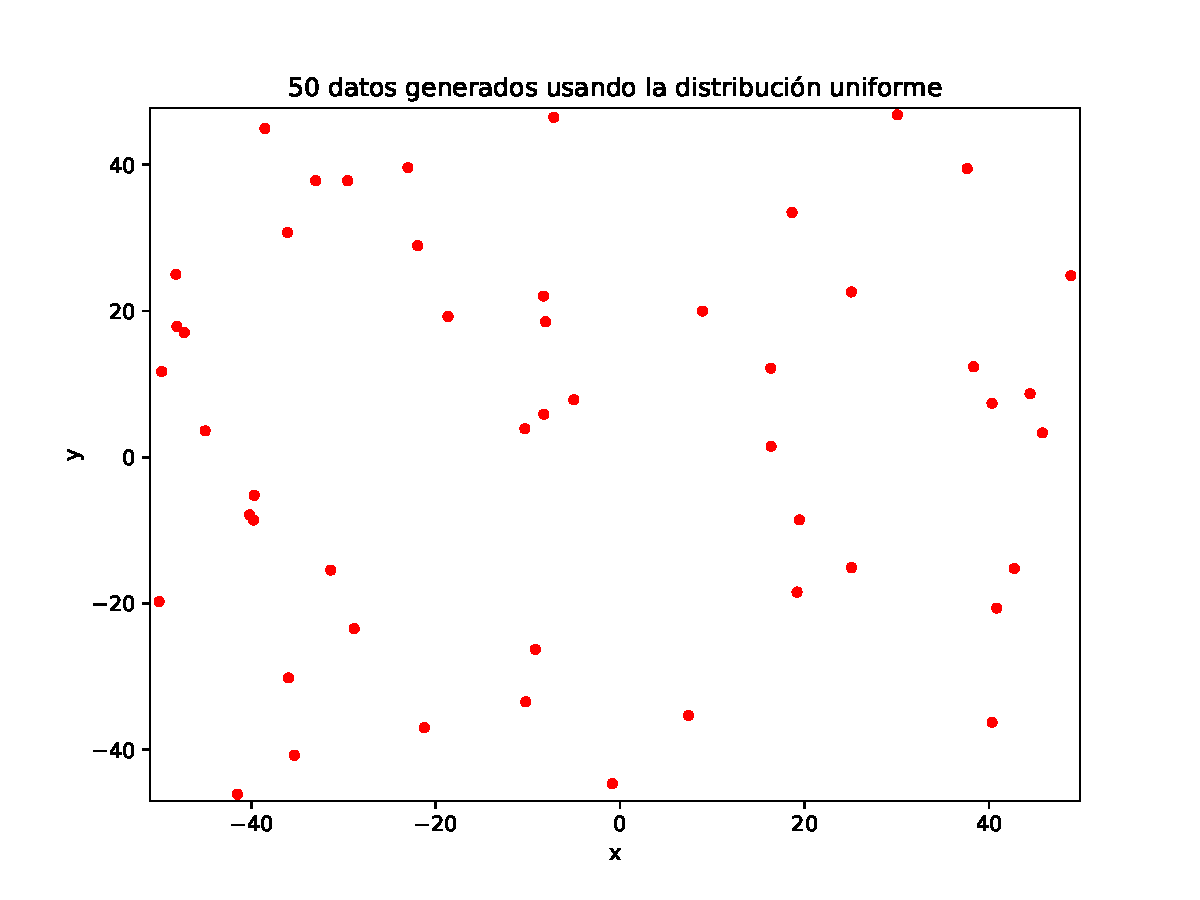
\includegraphics[scale = 0.4]{media/50-datos-uniforme.pdf}
\caption{Datos generados por la distribución uniforme en $[-50,50] \times [-50,50]$.}
\end{figure}

De igual manera, se pide generar datos pero usando la distribución normal o Gaussiana. Sabemos que en una distribución Gaussiana $X\sim \mathcal{N}(\mu,\sigma^2)$ , cuyos parámetros son la media $\mu$ y la varianza $\sigma^2$, la función de densidad viene dada por:
$$
F_{\mathcal{N}}(x) = \frac{1}{\sigma \sqrt{2\pi}} e^{- \frac{1}{2} \left(\frac{x - \mu}{\sigma}\right)^2}.
$$
Generamos de nuevo 50 valores en dos dimensiones. Para ello, se nos indica que $\sigma_x = \sqrt{5}$ y $\sigma_y = \sqrt{7}$. El resultado obtenido es el siguiente:
\begin{figure}[H]
  \centering
  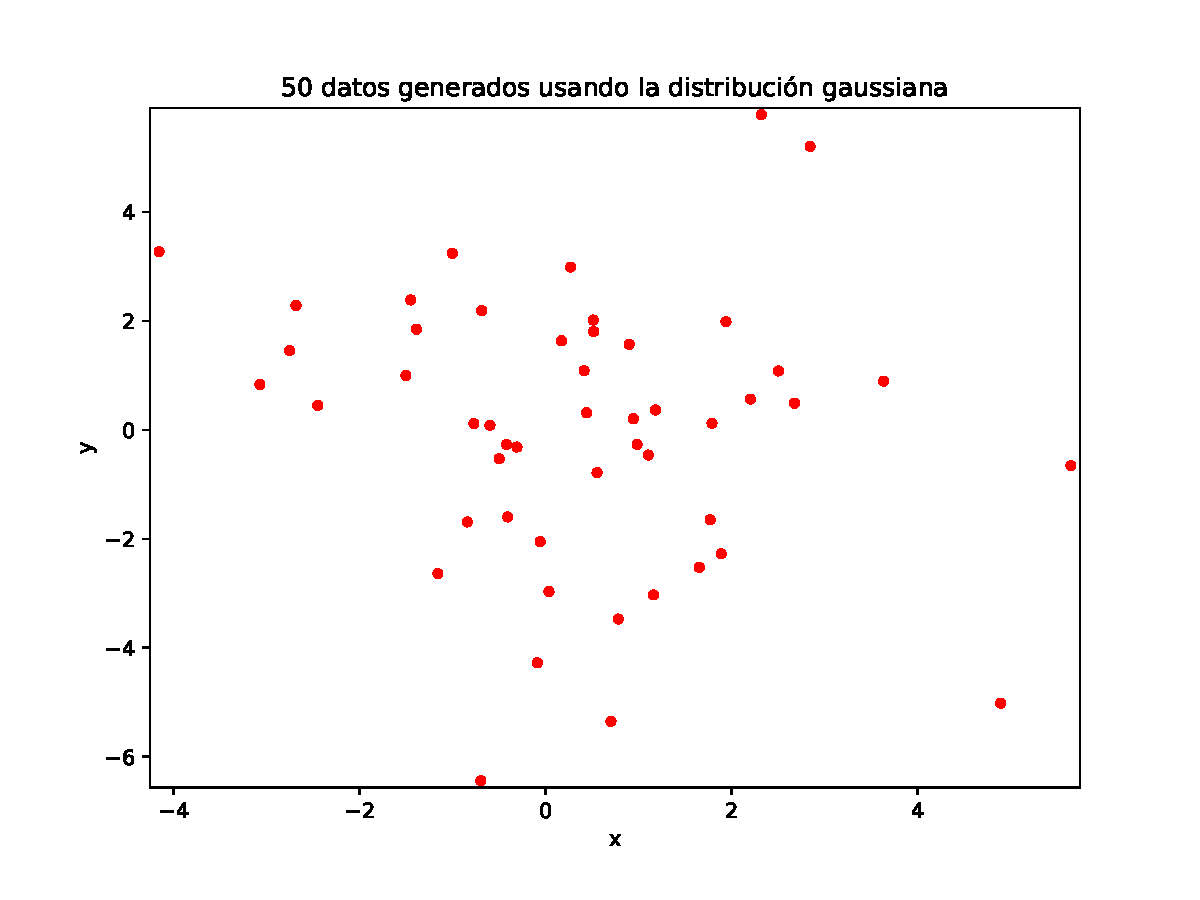
\includegraphics[scale = 0.4]{media/50-datos-gauss.pdf}
  \caption{Datos generados por la distribución normal en $[-50,50] \times [-50,50]$ con $\mu = 0, \sigma = (\sqrt{5},\sqrt{7})$.}
  \end{figure}
Como podemos ver, prácticamente la totalidad de los datos se encuentran en los intervalos conformados por 3 veces las desviaciones típicas de cada eje, esto es: $[-3 \sigma_x,3 \sigma_x] \times [-3 \sigma_y , 3 \sigma_y]$, como es esperado en esta distribución.\\


Una vez que hemos obtenido nuestros datos, vamos a proporcionarles unas etiquetas y vamos a introducir ruido en estos datos. Vamos primero a asignarle las etiquetas. Para ello, vamos generar una recta aleatoria usando la función dada (a la que le hemos cambiado el nombre) \lstlinlne{generate\_line(interval)} a la que le pasamos un intervalo $interval = [c,d]$, genera dos puntos en $\mathbb R^2$ dentro del cuadrado $[c,d]\times [c,d]$ y devuelve la pendiente $(a)$ y el término independiente $(b)$ de la recta que pasa por ellos. Una vez tenemos estos dos valores, sabemos que la recta es simplemente:
$$
y = ax + b.
$$
Considerando la función $f(x,y) = y- ax +b,$ obtenemos la distancia del punto $(x,y)$ a la recta, y podemos considerar como etiqueta el \textbf{signo} de esta distancia.
$$
f(x,y) = sign(y - ax - b).
$$
Se considera que los puntos que están sobre la recta son de la clase del $1$. Si dibujamos una recta aleatoria y dividimos 100 puntos generados mediante la distribución uniforme, obtenemos el siguiente gráfico:
\begin{figure}[H]
  \centering
  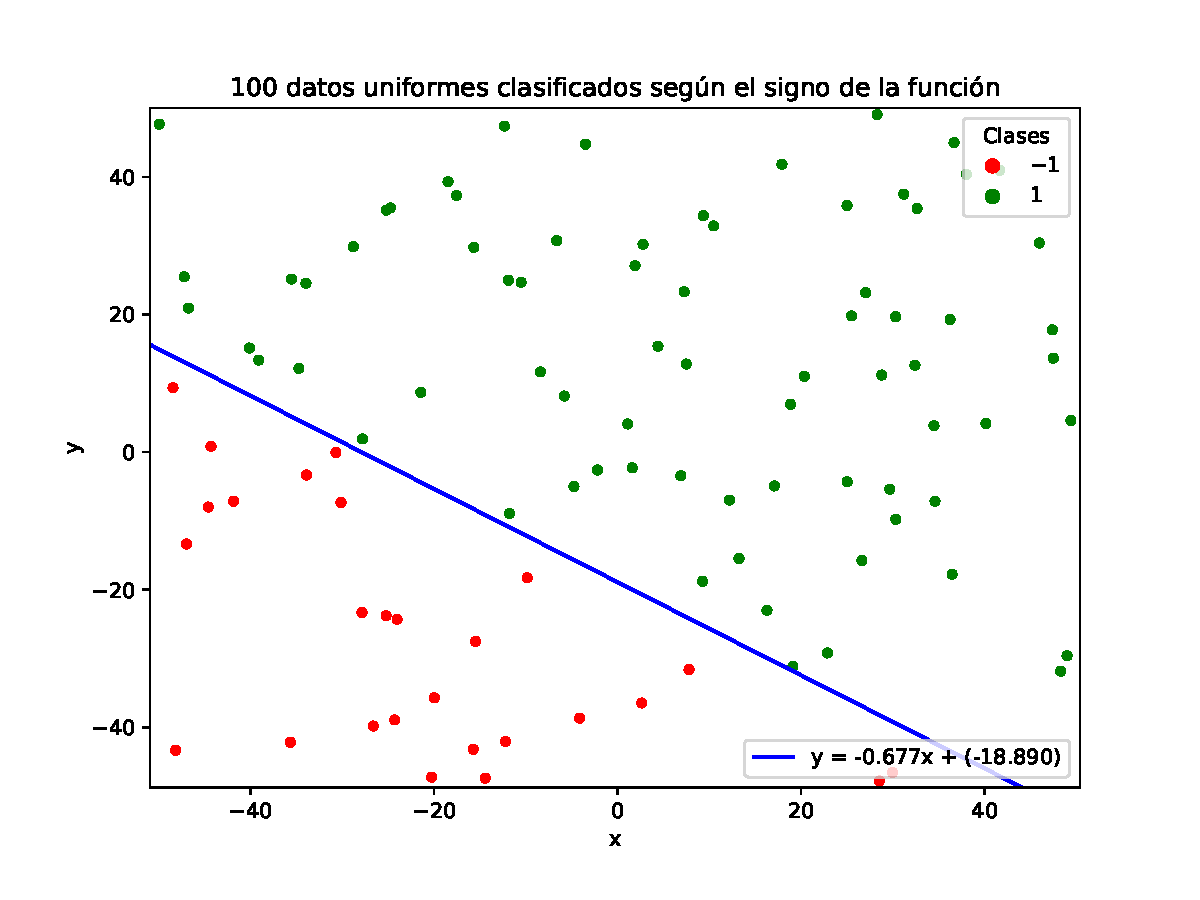
\includegraphics[scale = 0.4]{media/100-datos-separados.pdf}
  \caption{$100$ datos etiquetados mediante la separación por una recta aleatoria.}
\end{figure}

Nos toca entonces introducir ruido en estos datos.  Para ello, simplemente tomamos el vector de etiquetas \lstinline{y} de nuestros datos, obtenemos los índices de las etiquetas positivas  y de esas seleccionamos aleatoriamente un $10\%$ y las cambiamos a negativas. Hacemos lo mismo con las negativas. Esto se hace en la función \lstlinlne{generate\_noise}, cuyo código es simple:

\begin{lstlisting}[language=Python]
  def generate_noise(y,per = 0.1):
    
    ycopy = np.copy(y)

    for label in {-1,1}:
        # Get index of labels
        idx = np.where(y==label)[0]
        # Random selection of percentage*length labels
        changes = np.random.choice(idx,int(per*len(idx)),replace=False)
        # Change labels
        ycopy[changes] = -label
      
  return y_copy
\end{lstlisting}

Se realiza una copia de las etiquetas para mantener las originales. Si volvemos a dibujar los datos , el resultado es el siguiente:
\begin{figure}[H]
  \centering
  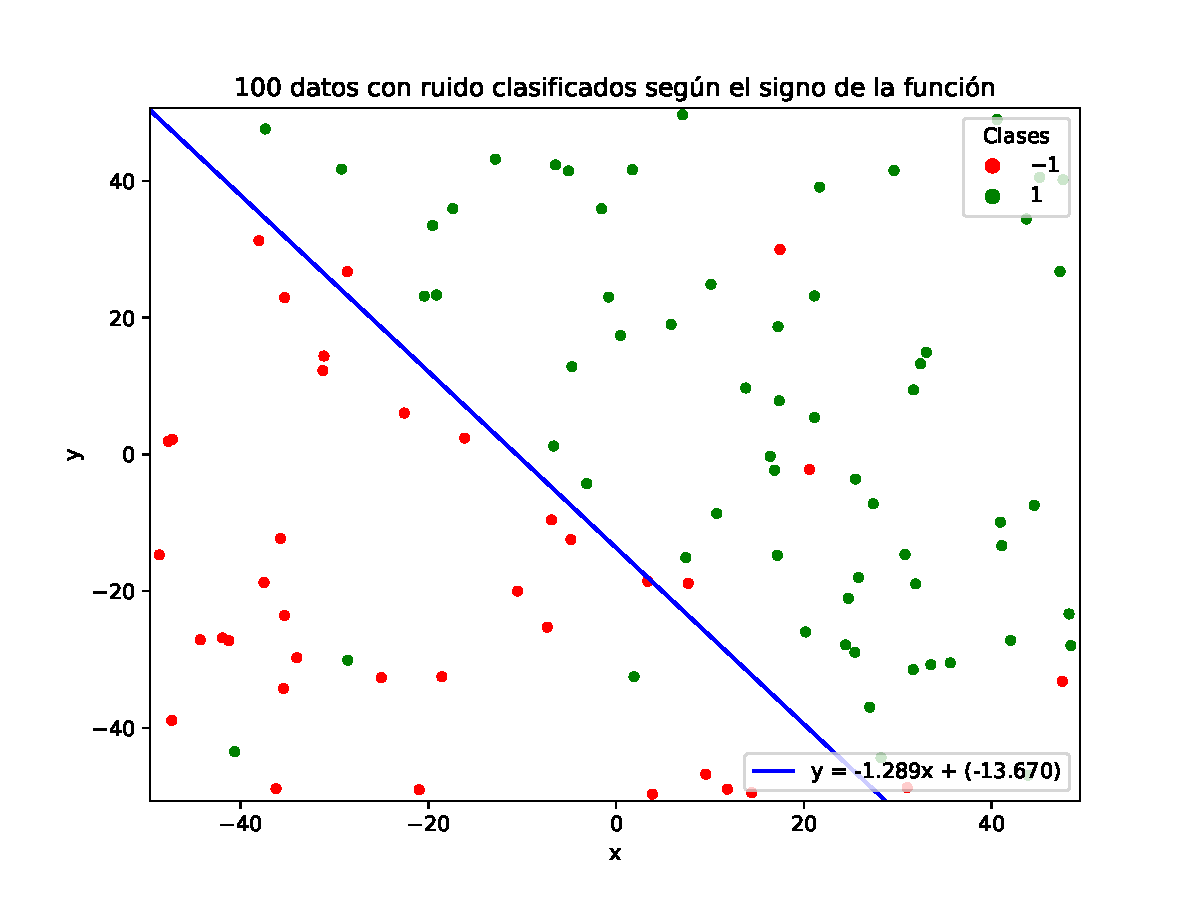
\includegraphics[scale = 0.4]{media/100-datos-ruido.pdf}
  \caption{$100$ datos etiquetados y con $10\%$ de ruido.}
\end{figure}
Como queríamos obtener, tenemos los puntos mal etiquetados respecto a la recta. 

Para continuar en este ejercicio, definimos las siguientes funciones:
\begin{itemize}
  \item $f(x,y) = (x-10)^2 + (y-20)^2 - 400$, que es una elipse.
  \item $f(x,y) = \frac{1}{2}(x+10)^2 + (y-20)^2 -400$, que es otra elipse.
  \item $f(x,y) = \frac{1}{2}(x - 10)^2 - (y+20)^2 -400$, que es una hipérbola.
  \item $f(x,y) = y - 20x^2 - 5x + 3$, que es una parábola clásica.
\end{itemize}
Estas serán nuestras nuevas funciones frontera de clasificación para la muestra. Sin embargo, ellas no definirán etiquetas para los puntos que generamos, sino que seguiremos usando las \textbf{etiquetas con ruido} del apartado anterior. Recordamos que la frontera con estas funciones podemos definirla igualando las expresiones a cero, y usando esto podemos dibujar las cuatro con lars regiones negativa y positiva para ver qué ocurre con los puntos etiquetados que habíamos generado:

\begin{figure}[H]
  \centering
  \subfloat[Primera elipse]{\label{fig:a}\includegraphics[width=0.45\linewidth]{media/Elipse1.pdf}}\qquad
  \subfloat[Segunda elipse]{\label{fig:b}\includegraphics[width=0.45\linewidth]{media/Elipse2.pdf}}\\
  \subfloat[Hipérbola]{\label{fig:c}\includegraphics[width=0.45\textwidth]{media/"Hipérbola".pdf}}\qquad%
  \subfloat[Parábola]{\label{fig:d}\includegraphics[width=0.45\textwidth]{media/"Parábola".pdf}}%
  \caption{Fronteras de clasificación. En verde zona positiva. En rojo, negativa.}
  \label{fig:myfig}
\end{figure}

Como se puede observar, ninguna de las funciones ajusta nada bien los datos que hemos generado inicialmente. Podemos tratar de justificar esto obteniendo la precisión (o \emph{accuracy}) de cada uno de ellos. Sabemos que esta viene dada por 
$$
Accuracy = \frac{TP + TN}{P + N}
$$
donde $TP$ es el número de ejemplos positivos que se han clasificado bien, $TN$ es el número de ejemplos negativos que se han clasificado bien, y $P,N$ son los números de positivos y negativos respectivamente. Además, si las clases no estuviesen balanceadas, existe una función que hace hace un accuracy ponderado al número de elementos de cada clase.Para calcular esto, \lstinline{sklearn} dispone de un conjunto de funciones que se encuentra en \lstlinline{sklearn.metrics}, y que son \lstinline{accuracy_score(y_true,y_predicted), balanced_accuracy_score(y_true, y_predicted)}. Los resultados que obtenemos al ejecutar un trozo de código que nos calcula para cada una de las funciones estos valores, son los siguientes:

\begin{table}[H]
  \centering
  \begin{tabular}{|l|l|l|}
  \hline
  Funcion    & Precisión & Precisión balanceada \\ \hline
  Recta      & $91$      & $89.51$              \\ \hline
  Elipse $1$ & $53$      & $42.62$              \\ \hline
  Elipse $2$ & $56$      & $47.79$              \\ \hline
  Hipérbola  & $30$      & $36.66$              \\ \hline
  Parábola   & $39$      & $51.58$              \\ \hline
  \end{tabular}
  \end{table}


Como ya nos indicaban las gráficas, las \textbf{precisiones} que obtienen las funciones dadas son muy bajas. Los cambios en la precisión balanceada se deben a que el número de datos no es igual en ambas clases, pues la recta deja más puntos a un lado que al otro. Además, la precisión de estos clasificadores es muy inferior a la que obtenemos por la recta, así que lo que podemos concluir es que si fuésemos a considerar alguno de estos clasificadores para nuestro conjunto de datos, los resultados serían obviamente mucho peores que los del clasificador lineal inicial. Por tanto, hemos visto que añadir complejidad al mdelo no implica que los resultados vayan a mejorar, por lo que es mejor usar el \textbf{clasificador lineal}. Esto además tiene mucho sentido en este caso, pues sabemos de antemano que las etiquetas han sido generadas usando este modelo lineal.

En cuanto al \textbf{ruido} que obtenemos en las etiquetas, debemos asumir que con datos reales esto es algo que pasará muy a menudo. Esto además influirá de forma muy directa en el aprendizaje, pues ocasiona que los datos \textbf{no sean separables} y tengamos que estar siempre tratando con aproximaciones o probabilidades de que nuestros clasificadores sean correctos, y obtener clasificadores que tengan error cero con datos reales es prácticamente imposible.


\section*{Modelos lineales}

\subsection*{Algoritmo Perceptron}

En este apartado, estudiaremos el algoritmo \emph{PLA} para el problema de clasificación binaria. Este algoritmo recibe dos vectores $X,y$ con los datos y las etiquetas y devuelve los coeficientes del hiperplano que separa completamente los datos. \\

Veamos este algoritmo en pseudocódigo. Si $h(x) = sign( w^T x + b)$ es la función que usamos para clasificar, y notamos momentáneamente como $y_x$ la etiqueta que corresponde al punto $x$, tenemos:


\begin{algorithm}[H]
  \SetAlgoLined
  \KwResult{Hiperplano separador}

   $w \leftarrow$ inicialización

   \While{$w$ cambie}{
    \For{ $x \in X$}{ 
      \If{$h(x)$ no es igual a $ y_x$}{ 
        $w \leftarrow w + etiqueta(x)\cdot x$
      }
    }
   }
    \Return{w}
   \caption{Algoritmo Perceptron ( $X$, $y$, $maxIter$)}
  \end{algorithm}
  
Como vemos, si la etiqueta que nuestros pesos están produciendo no es la correcta, esto es, si $h(x) \neq y_x$,  actualizamos en cada iteración $w$ de la forma:
$$
w(t+1) = w(t) + x \cdot y_x,
$$
y realizamos esta operación tantas veces como sea necesario hasta que no haya ningún cambio en los pesos, es decir, todos los puntos del conjunto de datos estén bien clasificados. Es claro que para que este algoritmo termine , los datos deben ser \textbf{linealmente separables} pues, de lo contrario, para cualesquiera pesos obtendríamos que existe un punto $x \in X$ para el cual $h(x) \neq y_x$, por lo que nuestro algoritmo iteraría indefinidamente. De hecho, se sabe que de por sí es un algoritmo muy costoso pues, si los datos son separables, encontrará la solución pero:

\newcommand{\norm}[1]{\left\lVert#1\right\rVert}

\textbf{Proposición.-} Si $B = \min \{ \norm{w} : y_i w^T \geq 1,\quad w \in \mathbb R^d\}$ y $R = \max_{i} \norm{x_i}$, entonces PLA encontrará la solución óptima en, a lo sumo:
$$
(RB)^2 \text{ iteraciones}
$$
Esto puede ser un número muy elevado según las dimensiones de los datos. Es por ello que, para cuando trabajemos con datos con ruido, hemos establecido un número máximo de iteraciones a realizar, \lstinline{max_iter = 1000}, pues sabemos que nunca encontrará los pesos que separen los datos.\\



Una vez explicado, vamos a pasar a ejecutar el algoritmo. Lo hacemos primero usando los \textbf{datos sin ruido} de la sección anterior.
\begin{itemize}
\item Si inicializamos con el vector $w_0 = (0,0,0)$, obtenemos lo siguiente:
\begin{lstlisting}[language=bash]
  Pesos obtenidos para peso inicial [0,0,0]: [564.          65.01749303  50.37298718]
  Iteraciones para peso inicial [0,0,0]: 105
  Accuracy = 100.0
\end{lstlisting}
Como podíamos esperar, el resultado es perfecto y el número de iteraciones es pequeño.

\item Ahora, se pide que se inicialice el vector de pesos inicial $w_0$ con valores aleatorios entre $0$ y $1$. Para ello, usando \lstinline{np.random.uniform(0,1,3)} obtenemos esos vectores aleatorios (esta es la función que usa \lstinline{generate_uniform_data}, por lo que podríamos haberla usado). Se pide que se repita el experimento $10$ veces y se dé el valor medio de las ejecuciones, y el resultado obtenido es el siguiente:
\begin{lstlisting}[language=bash]
  Valor medio de iteraciones necesario para converger: 112.7
  Valor medio de accuracy en pesos aleatorios: 100.0
  La desviación típica en las iteraciones ha sido: 6.664082832618455, pues las iteraciones son: [110, 122, 109, 112, 111, 112, 107, 103, 127, 114]
\end{lstlisting}
Como podemos ver, se ha dado un muy leve incremento en el número de iteraciones necesarias para encontrar los mejores pesos, y tenemos una desviación típica de $\approx 6$, lo cual no es despreciable por lo que no podemos indicar que inicializar los pesos aleatoriamente pueda ser mejor que inicializarlos a cero, ya que no nos garantiza que tengamos menos iteraciones para encontrar la solución.
\end{itemize}

Vamos a analizar ahora el caso en el que usamos los \textbf{datos con ruido}. Usamos los datos y etiquetas obtenidos en el ejercicio anterior y vamos a ver qué ocurre y tratar de dar una explicación al resultado. Si ejecutamos el mismo código que antes pero con las etiquetas con ruido, obtenemos el siguiente resultado:

\begin{lstlisting}[language=bash]
  Iteraciones para peso inicial [0,0,0]: 1000
  Accuracy = 73.0
  Resultados medios para 10 pesos iniciales aleatorios:
  Valor medio de iteraciones necesario para converger: 1000.0
  Valor medio de accuracy en pesos aleatorios: 85.5
  La desviación típica en las iteraciones ha sido: 0.0, pues las iteraciones son: [1000, 1000, 1000, 1000, 1000, 1000, 1000, 1000, 1000, 1000]
\end{lstlisting}

Observamos que en todos los casos, se han hecho todas las iteraciones posibles que habíamos marcado como tope. Pero, esto era bastante previsible. Hemos comentado anteriormente que para que \emph{PLA} siempre obtiene la solución que tiene error cero \textbf{si, y solo si,} los datos sobre los que se aplica son \textbf{separables}. En este caso, los datos no son separables debido al ruido, por lo que nuestro algoritmo seguirá iterando infinitamente tratando de encontrar el hiperplano que clasifique bien a todos los puntos pero no será capaz de encontrarlo. En todas las épocas habrá puntos que no estén bien clasificados y por tanto se seguirá actualizando los pesos e iterando. 

Guardando los pesos que se obtienen en cada época, podemos ver el error que se obtiene:

\begin{figure}[H]
  \centering
  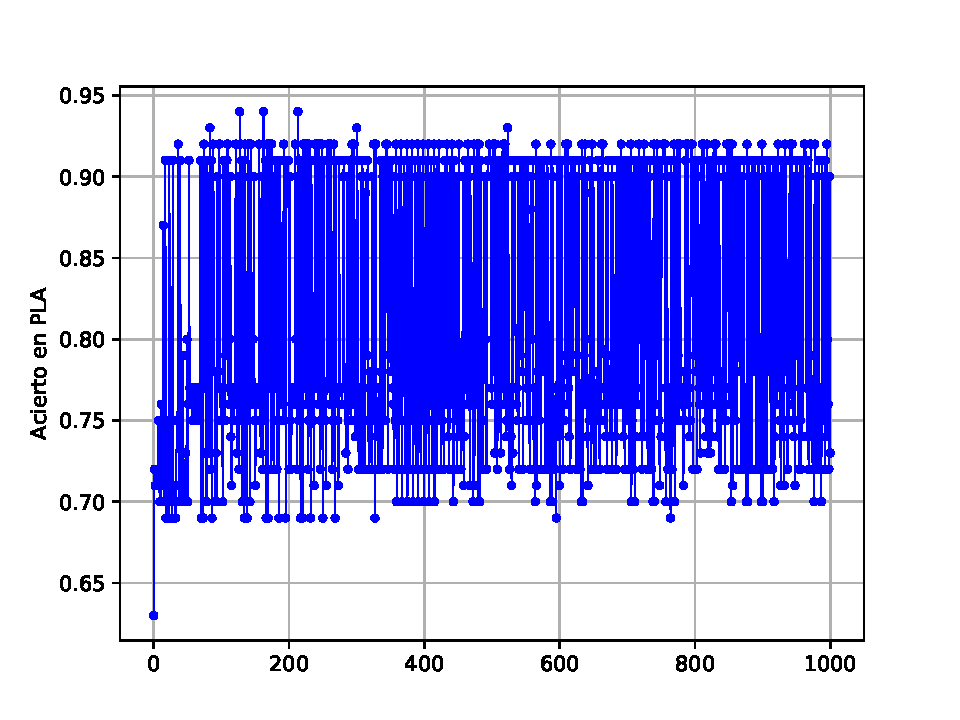
\includegraphics[scale = 0.6]{media/PLA-ruido.pdf}
  \caption{Porcentaje de acierto en datos con ruido por cada época usando \emph{PLA}.}
\end{figure}
El porcentaje de acierto va variando de manera muy brusca según las épocas, y no consigue en ningún momento converger, como esperábamos.

\subsection*{Regresión logística}

Hasta ahora, habíamos trabajado siempre con etiquetas determinísticas. Es decir, para cada dato $x\in X$, producíamos una etiqueta $y_x \in \{-1,1\}$. En \textbf{regresión logística}, vamos a producir una \emph{probabilidad} $p \in [0,1]$.

En la regresión lineal, obteníamos las etiquetas del siguiente modo:
$$
f(x) = \sigma_{lin}(w^T x) \quad \text{con} \quad \sigma_{lin}(a) = sign(a).
$$
Ahora, para la regresión lineal, utilizaremos una nueva función $\sigma$, llamada función logística, que viene dada por 
$$
\sigma(t) = \frac{1}{1 + e^{-t}},
$$
que siempre toma valores en el intervalo $[0,1]$. Por tanto, ahora lo que estamos obteniendo con esta $f(x)$ es la probabilidad de que $x$ pertenezca a la clase positiva $+1$, esto es:
$$
f(x) = \mathbb P [ y = +1 \ | \ x].
$$
Tenemos que definir por tanto también una función de error para ver cómo de bueno es nuestro modelo. Usando el método de \emph{máxima verosimilitud}, trataremos de seleccionar $h$ de nuestro conjunto de hipótesis $\mathcal H$ que , dado un conjunto de datos $X = \{(x_1,y_1),\dots,(x_n,y_n)\}$ maximice la probabilidad de que se den todas las etiquetas correctas para esos datos usando $h$, esto es $\prod_{i = 1}^N P(y_n \ | \ x_n)$. Sabemos que maximizar esa probabilidad equivale a minimizar el siguiente error:
\[
E_{\operatorname{in}}(w) = \frac{1}{N} \sum_{n=1}^N \ln \left( 1 + e^{-y_n w^T x_n}\right).  
\]
Puesto que la técnica que utilizaremos para minimizar esta función de error será el gradiente descendente estocástico (SGD), es necesario denotar que la derivada de esta función viene dada por:
\[
\nabla E_{\operatorname{in}}(w) = - \frac{1}{N} \sum_{n = 1}^N \frac{y_n x_n}{ 1 + e^{y_n x^T x_n}}.
\]
En nuestro caso, como usaremos SGD, lo evaluaremos punto a punto actualizando los pesos según el error en cada punto. 

El Gradiente Descendente Estocástico será implementado con las siguientes condiciones:
\begin{itemize}
  \item Los pesos iniciales serán el vector cero.
  \item El algoritmo dejará de iterar cuando la distancia entre los pesos de la época actual y la anterior sea menor que un $\epsilon$, que fijaremos a $\epsilon = 0.01$.
  \item Se aplicará una permutación del orden de los datos antes de usarlos en cada época del algoritmo.
  \item La tasa de aprendizaje se fija a $\eta = 0.01$.
\end{itemize}


Una vez que hemos plantado las condiciones, vamos a realizar el siguiente experimento: 
\begin{enumerate}
\item Generamos $N = 100$ puntos aleatorios y una recta = $y = ax + b$. Etiquetamos los puntos usando el signo de la distancia del estos puntos a la recta.

\begin{lstlisting}[language=Python]
  # Generate data and line
  a,b = generate_line([0,2])
  X = generate_uniform_data(N_train,2,[0,2])
  # Create tags using the line
  y = np.array([f(x[0],x[1],a,b) for x in X])
  X = np.hstack((np.ones((X.shape[0], 1)), X))
\end{lstlisting}

\item Aplicamos el algoritmo \lstlinline{sgdRL} que realiza la regresión logística para obtener los pesos de la recta que aproxima nuestros datos. Recordamos que en Gradiente descendente, la actualización de los pesos se hace en cada paso de la forma:
$$
w(t+1) = w(t) - \eta \cdot \nabla E_{\operatorname{in}}(w).
$$

\item Generamos un conjunto de test $X_{\operatorname{test}}$ de $N_{\operatorname{test}} = 1000$ puntos nuevos, y los etiquetamos con la misma función que etiquetamos los puntos que utilizamos para el entrenamiento.

\item Calculamos el error en el conjunto de test con la función de error logística. 

\end{enumerate}

Para este ejercicio podía haber dos interpretaciones: o bien fijar el conjunto de test y la recta que genera los datos , y generar en cada iteracion solamente nuevos conjuntos de entrenamiento, o generar en cada iteración nuevos conjuntos de entrenamiento, nueva recta y nuevo conjunto de test. Hemos elegido la segunda forma.\\

Elegimos esta forma de realizar el experimento generando en cada iteración nuevos datos de entrenamiento pues tiene más interés que el otro caso, ya que si fijásemos tanto una recta como un conjunto de test, los resultados que se obtendrían serían más bien \emph{relativos} a cómo actúa la regresión logística respecto a esa recta fijada y ese conjunto de test fijado (aunque arbitrario). Sin embargo, al elegir \textbf{variar} tanto la recta como el conjunto de test, consideramos que se obtiene una idea más general de cómo de bien funciona esta regresión logística cuando los todos los conjuntos son arbitrarios, y la información que nos da es relativa a cómo se comporta en general la regresión logística cuando tenemos unos datos distribuidos de manera uniforme, caso más general que el anterior.

Vamos a ejecutar el experimento una única vez para ver cómo ajusta la recta obtenido al conjunto de datos de test $X_{\operatorname{test}}$. El resultado  tanto dentro como fuera de la muestra es el siguiente:
\begin{figure}[H]
  \centering
  \subfloat[Regresión Logística sobre conjunto de entrenamiento.]{\label{fig:a}\includegraphics[width=0.45\linewidth]{media/"LR vs Original-Train-eps0.01".pdf}}\qquad
  \subfloat[Regresión Logística fuera de la muestra de entrenamiento.]{\label{fig:b}\includegraphics[width=0.45\linewidth]{media/"LR vs Original-eps0.01".pdf}}
  \caption{Regresión logística sobre $N=100$ datos de muestra y sobre nueva muestra de $1000$ datos. }
  \label{fig:myfig:2}
\end{figure}
El ajuste como podemos ver es casi perfecto, aunque algún dato queda mal clasificado. Si mostramos por pantalla el error en la muestra, el resultado es:
\begin{lstlisting}[language=bash]
  El error en la muestra es de [0.10090145751031432]
  Average results in 1 experiments:
         Iterations: 400.0
         Error Eout: 0.09428134264702463
\end{lstlisting}

Lo cual nos indica que , como podíamos ver, es bajo pero no es cero. Esto es debido a que la diferencia entre los pesos en dos iteraciones ha sido muy pequeña aunque estos no ajusten perfectamente a los datos. Si le diésemos un número mayor de iteraciones o estableciésemos otra condición de parada con un epsilon menor, es posible que obtuviésemos un mejor ajuste de los datos, aunque con un mayor número de iteraciones. Aunque no sea el objetivo del ejercicio, se ha realizado una prueba de esto para ver si esto era cierto y el resultado es el siguiente:

\begin{figure}[H]
  \centering
  \subfloat[Regresión Logística sobre conjunto de entrenamiento.]{\label{fig:a}\includegraphics[width=0.45\linewidth]{media/"LR vs Original-Train-eps0.005".pdf}}\qquad
  \subfloat[Regresión Logística fuera de la muestra de entrenamiento.]{\label{fig:b}\includegraphics[width=0.45\linewidth]{media/"LR vs Original-eps0.005".pdf}}
  \caption{Regresión logística con epsilon menor. Iteraciones necesarias: $1168$. }
  \label{fig:myfig:3}
\end{figure}
Se obtiene que el error en la muestra es $E_{in} = 0.0971$ y el error en el conjunto de test es $E_{out} = 0.10273$ con lo que, aunque hemos mejorado el error en la muestra, hemos empeorado fuera de ella, se ha producido un sobreajuste (overfitting). Además, se han incrementado razonablemente las iteraciones, como vemos en el pie de la figura \ref{fig:myfig:3}.\\

Por último, lo que haremos será \textbf{repetir este experimento} $N_{experiments} = 100$ veces y calcular la media de los errores fuera de la muestra y el número medio de iteraciones, para hacernos una idea de cómo de bien funciona la regresión logística sobre los datos generados de esta forma. El resultado de la ejecución de este experimento es el siguiente:
\begin{lstlisting}[language=bash]
  Average results in 100 experiments:
         Iterations: 414.95
         Error out sample: 0.12018870542312315
\end{lstlisting}

\newpage
Observamos que el número de iteraciones no es muy alto para obtener unos pesos que ajusten razonablemente bien nuestros datos incluso fuera de la muestra, obteniendo un error de $0.12$. Esta información es bastante escueta, así que decidimos imprimir por pantalla también los siguientes datos.

\begin{lstlisting}
Average Error in sample: 0.1095453701333863
Desviación típica iteraciones: 77.46565367955014
Desviación típica E_out: 0.02063634008621514
\end{lstlisting}

Vemos qué nos dice cada uno:
\begin{itemize}
  \item Que el error medio en la muestra $E_{\operatorname{in}}$ sea de $0.109$ nos indica que por lo general la muestra no es fácil de ajustar. Además, podemos ver que el error medio en la muestra no queda muy lejos del error medio fuera de la media , lo que nos indica que el ajuste que estamos haciendo generaliza razonablemente bien.
  
  \item Tenemos que la desviación típica de las iteraciones es $\approx 77$. Esto nos indica que hay un rango grande de iteraciones que tarda el algoritmo en converger. Esto es debido a que hay muestras que deben ser bastante más complicadas de ajustar que otras.
  \item Por último, tenemos una desviación típica del error fuera de la muestra $E_{\operatorname{out}} $ de aproximadamente $0.02$. Esto indica que todos los pesos que obtenemos como resultado de la regresión logística ajustan razonablemente bien fuera de la muestra, no hay unos que ajusten muy bien y otros que ajusten muy mal.
\end{itemize}

Como conclusión a estos datos obtenidos, podemos decir que nuestro modelo en este tipo de distribuciones consigue generalizar de forma bastante correcta.

\section*{Bonus - Clasificación de Dígitos}

Consideramos el conjunto de datos de dígitos manuscritos en los que hemos restringido a aquellos cuya etiqueta es $4$ u $8$. Vamos a utilizar las características \emph{intensidad promedio} y \emph{simetría} igual que hicimos en la práctica anterior para clasificar dígitos. Comenzamos planteando el problema de clasificación , identificando sus elementos:
\begin{itemize}
\item Tendremos el conjunto de datos $\mathcal X$. Este se crea del siguiente modo: primero, se seleccionan aquellas parejas $(x_i,y_i)$ en las cuales $y_i \in \{4,8\}$. Una vez seleccionados, nos quedamos con dos características que son simetría e intensidad promedio, por lo que nos estamos quedando con $x_i \in \mathbb R^2$. Para homogeneizar los datos como hicimos en la práctica anterior, añadiremos un $1$ como primera componente de cada dato $x_i$, por lo que nuestro espacio final de características será:
$$
\mathcal X = \{1\} \times \mathbb R^2
$$
\item Tendremos las etiquetas $y_i \in \{4,8\}$ que indicarán para un vector de características $x_i$, el dígito al que pertenece, ya sea el $4$ u el $8$. Para la comodidad en la clasificación, identificaremos el $4$ como la etiqueta $-1$, y el $8$ como la etiqueta $1$. Por tanto, $\mathcal Y = \{-1,1\}$.

\item Juntando los dos anteriores, obtenemos nuestro conjunto de entrenamiento que será:
$$
\mathcal D = \{(x_n,y_n) \ : x_n \in \mathcal X, y_n \in \mathcal Y, n = 1,\dots,N\}
$$
con un total de $N = 1194$ datos.

\item Tenemos la función objetivo $f: \mathcal X \to \mathcal Y$ es la función de etiquetado que queremos encontrar, es desconocida. 

\item La clase de funciones $\mathcal H$ que usaremos para buscar nuestra $f$ sí que la conocemos, y será la clase de las funciones lineales de $\mathbb R^3$ en $\mathbb R$, que además clasifican a los datos al conjunto $\{-1,1\}$. Por tanto, podemos definirla formalmente como:
$$
\mathcal H = \left\{h : \mathbb R^3 \to \mathbb R \ | \ h(x) = signo(w^T x), \ w \in \mathbb R^3\right\}
$$

\item La técnica que se usaremos es la minimización del riesgo empírico (ERM) para hallar la función $g$ en nuestra clase de funciones que haga que el error de la muestra sea mínimo. Este error, recordamos que si $h \in \mathcal H$, es:
$$
E_{\operatorname{in}}(h) = \frac{1}{N} \sum_{n = 1}^N [[ h(x_n) \neq y_n]]
$$

\item Como algoritmos $\mathcal A$, usaremos un modelo de regresión lineal, que luego intentaremos mejorar utilizando \lstinline{PLA-Pocket}, que será comentado brevemente más adelante.

\item Para evaluar la bondad de nuestro modelo, tenemos un conjunto de \emph{test} dado, que tiene $366$ datos definidos de la misma forma que se definen para el conjunto de entrenamiento.


\end{itemize}

Con estos elementos, queda bien definido nuestro problema y podemos pasar a explicar los modelos que usaremos. 
\begin{enumerate}
\item Como modelo de \textbf{regresión lineal}, utilizaremos el algoritmo de \textbf{pseudoinversa}, ya que lo utilizamos en la práctica anterior y, aunque no esté computado por la descomposición \emph{SVD}, para este conjunto de datos pequeño es más que suficiente el código que ya teníamos implementado.

\item Aplicaremos posteriormente el algoritmo \lstlinline{PLA-Pocket}. Este no es más que el mismo \textbf{PLA} que hemos aplicado en los apartados anteriores, solo que almacenando \emph{``en el bolsillo''} el vector de pesos que se ha obtenido en alguna de las iteraciones y es el mejor en toda la muestra, es decir, el que menor error de clasificación nos proporciona. Esta solución, por supuesto, no soluciona el problema de que si los datos no son linealmente separables entonces no se encontrará el hiperplano separador. Sin embargo, se consigue que la solución no proporcione peores resultados conforme avanzan las iteraciones, es decir, no empeore con el tiempo.

\end{enumerate}


Vamos primeramente a visualizar los conjuntos de entrenamiento y de test, para ver cómo son nuestros conjuntos de datos. El resultado es el siguiente:
\begin{figure}[H]
  \centering
  \subfloat[Conjunto de Train.]{\label{fig:a}\includegraphics[width=0.45\linewidth]{media/"Digitos-Manuscritos-Train".pdf}}\qquad
  \subfloat[Conjunto de Test.]{\label{fig:b}\includegraphics[width=0.45\linewidth]{media/"Digitos-Manuscritos-Test".pdf}}
  \caption{Conjuntos de train y test para el problema de clasificación de dígitos $4$ y $8$.}
\label{fig:myfig:4}
\end{figure}

Como podemos observar, estos datos son claramente \textbf{NO separables}. El algoritmo de \emph{pseudoinversa} nos proporcionará el mínimo teórico que podemos alcanzar según la minimización del riesgo empírico. Sin ambargo, si quisiésemos aplicar aquí el algoritmo \lstinline{PLA} tendríamos un problema, pues nunca encontraríamos una solución debido a la no separabilidad de los datos. Es por ello que aplicar \lstinline{PLA-Pocket} ahora tiene bastante sentido, pues podemos apreciar si es una mejora al algoritmo \lstinline{PLA},ya que este podría obtener una solución que sea razonablemente parecida a la que nos da el algoritmo de pseudoinversa al ser capaz de guardar el mejor de los pesos. 

Primero, observamos cómo se comporta el algoritmo de pseudoinversa sobre los datos:
\begin{figure}[H]
  \centering
  \subfloat[Clasificación usando pseudoinversa en train.]{\label{fig:a}\includegraphics[width=0.45\linewidth]{media/"Pseudoinverse-train".pdf}}\qquad
  \subfloat[Clasificación usando pseudoinversa en train.]{\label{fig:b}\includegraphics[width=0.45\linewidth]{media/"Pseudoinverse-test".pdf}}
  \caption{Clasificación usando pseudoinversa en train y test.}
\label{fig:myfig:4}
\end{figure}
Además, podemos calcular el \emph{porcentaje de error} en ambos conjuntos para pseudoinversa, para en el futuro comparar. El resultado es:
\begin{lstlisting}[language=bash]
  El porcentaje de error de pseudoinversa es:
	 Train: 22.78057%
	 Test: 25.13661%
\end{lstlisting}
Los resultados no son tan buenos como serían si los datos fuesen separables, tenemos un error de casi 1 de cada 4 datos, lo cual es bastante elevado.\\

Vamos a ver qué ocurre cuando ejecutamos el algoritmo \lstinline{PLA-Pocket}.  Comenzamos inicializando los pesos del algoritmo de forma aleatoria. A priori, como los datos no son separables, ya sabemos que el algoritmo no va a encontrar ningún hiperplano que nos de error cero. Sin embargo, es interesante ver cuánto se acerca este algoritmo a la solución dada por la pseudoinversa. El resultado gráfico es el siguiente:
\begin{figure}[H]
  \centering
  \subfloat[Clasificación usando PLA-Pocket en train.]{\label{fig:a}\includegraphics[width=0.45\linewidth]{media/"PLA-Pocket-Random-Ini-train".pdf}}\qquad
  \subfloat[Clasificación usando PLA-Pocket en test.]{\label{fig:b}\includegraphics[width=0.45\linewidth]{media/"PLA-Pocket-Random-Ini-test".pdf}}
  \caption{Clasificación usando PLA-Pocket con inicialización aleatoria en train y test.}
\label{fig:myfig:4}
\end{figure}

Podemos ver como el ajuste parece también razonablemente bueno, parecido al del algoritmo anterior. Podemos ver el error tanto en la muestra como en el conjunto de test que produce el algoritmo:
\begin{lstlisting}[language=bash]
  El porcentaje de error de PLA-Pocket pesos iniciales aleatorios es:
        Train: 22.61307%
        Test: 25.68306%
\end{lstlisting}

Este algoritmo obtiene unos errores muy parecidos al caso anterior. 
Como podemos apreciar, hemos mejorado un poco el porcentaje de acierto  en el conjunto de train y hemos mantenido el error en el conjunto de test. Como las rectas son visualmente
prácticamente idénticas y el número de puntos en el conjunto de test no es muy grande, estos resultados son lógicos.

Por último, una buena idea para \lstinline{PLA-Pocket} puede ser inicializar el algoritmo con los pesos que nos proporciona la regresión lineal y ver si es capaz de mejorar los resultados 
que esta regresión ha obtenido. A priori, parece una buena idea comenzar directamente con unos pesos que sean razonablemente buenos, guardarlos como los mejores e ir haciendo modificaciones pequeñas sobre ellos para ver si se encuentran algunos que sean mejores dentro de la muestra, y luego probarlos a ver qué tal se comportan fuera de la muestra.  Tras ejecutar el código anterior pero inicializando con los pesos que nos da el algoritmo de pseudoinversa, el resultado es el siguiente:
\begin{lstlisting}[language=bash]
  El porcentaje de error de PLA-Pocket pesos iniciales dados por pseudoinversa es:
         Train: 22.52931%
         Test: 25.40984%
\end{lstlisting}

%Como vemos, el resultado es exactamente el mismo en el caso anterior. Podemos ver los pesos que devuelven los algoritmos:
%%\begin{lstlisting}[language=bash]
%%  Pesos pseudoinversa: [-0.50676351  8.25119739  0.44464113]
%%  Pesos PLA: [ -7.27402697 138.48932567   7.61929994]
%%  Pesos Pseudo+PLA :[ -8.50676351 163.00130454   8.99007863]  
%%\end{lstlisting}
%Los pesos son diferentes en todos los casos, pero aún así los resultados que obtenemos son bastante parecidos o iguales. De hecho, si dibujamos las rectas que hemos obtenido en este caso:

\begin{figure}[H]
  \centering
  \subfloat[Clasificación usando Pseudoinversa + PLA-Pocket en train.]{\label{fig:a}\includegraphics[width=0.45\linewidth]{media/"PLA-Pocket-Pseudo-Ini-train".pdf}}\qquad
  \subfloat[Clasificación usando Pseudoinversa +PLA-Pocket en test.]{\label{fig:b}\includegraphics[width=0.45\linewidth]{media/"PLA-Pocket-Pseudo-Ini-test".pdf}}
  \caption{Clasificación usando PLA-Pocket, con inicialización con pesos iniciales de pseudoinversa, en train y test.}
\label{fig:myfig:5}
\end{figure}
Podemos ver que son prácticamente iguales a las anteriores a simple vista. Para ver esto mejor, vamos a realizar el gráfico de las 3 rectas juntas para ver qué resultado obtenemos:

\begin{figure}[H]
  \centering
  \subfloat[Todas las rectas en train.]{\label{fig:a}\includegraphics[width=0.45\linewidth]{media/compBonusTrain.pdf}}\qquad
  \subfloat[Todas las rectas en test.]{\label{fig:b}\includegraphics[width=0.45\linewidth]{media/compBonusTest.pdf}}
  \caption{Rectas obtenidas por regresión lineal, PLA-Pocket (inicialización aleatoria), y PLA-Pocket (inicialización con pesos de regresión) .}
\label{fig:myfig:6}
\end{figure}


\subsubsection*{Cotas del error $E_{\operatorname{out}}}$}

Nos quedaría por calcular las cotas sobre el verdadero valor de $E_{\operatorname{out}}$, basándonos tanto en $E_{\operatorname{in}}$ como en $E_{\operatorname{test}}$.  Para esto, aplicaremos primero la desigualdad de Hoeffding que sabemos que, dado $N$ el tamaño del conjunto de datos y $\delta > 0$ el nivel de confianza, tenemos que:
$$
E_{\operatorname{out}}(g) \leq E_{\operatorname{in}}(g) + \sqrt{\frac{1}{2N} \log \frac{2 \abs{\mathcal H}}{ \delta}}
$$
con probabilidad mayor o igual que $1- \delta$.

Vamos a aplicarla a nuestro caso. Basándonos primero en el error en la muestra $E_\operatorname{in}$, tenemos que el tamaño de la clase de funciones es infinito, por lo que a priori no podríamos calcular esta cota. Sin embargo, al estar trabajando con nuestro ordenador y sabiendo que cada flotante en nuestro ordenador son $64$ bits, entonces podemos decir que $\abs{H} \approx 2^{64\dot 3}$, pues utilizamos 3 valores reales para los vectores de pesos. Por tanto, podemos programar la cota con la siguiente función simple:

\begin{lstlisting}[language=Python]
  def Hoeffding_bound(in_sample_error,N,card_h = 2**(64*3),delta = 0.005):
    return in_sample_error + np.sqrt( (1/2*N) * np.log( (2*card_h)/delta) )
\end{lstlisting}

Cada uno de los vectores de pesos nos proporciona unos errores en la muestra como hemos visto anteriormente. Si ejecutamos esta desigualdad usando el error en la muestra, con el $N$ que hemos indicado en el enunciado del problema, el resultado que obtenemos es el siguiente:
\begin{lstlisting}
  Cota del error E_out por desigualdad de Hoeffding usando E_in según algoritmo:
    Pseudoinversa: E_out <= 0.46713
    PLA-Pocket-Random inicialización: E_out <= 0.46713
    PLA-Pocket-Pseudoinversa inicialización: E_out <= 0.46462
\end{lstlisting}
Donde vemos que el algoritmo \lstinline{PLA-Pocket} mejora un poco la cota del algoritmo de pseudoinversa, pues partiendo del mismo hiperplano que esta, intenta seguir minimizando usando un error diferente al error cuadrático medio que es el que se minimiza con la pseudoinversa. 

Ahora, veamos qué ocurre si acotamos el error fuera de la muestra mediante el error en el conjunto de test. Para ello, calculamos el error $E_{\operatorname{test}}$ con cada uno de los algoritmos y, como en test ya hemos escogido la función objetivo $g$ pues ya tenemos los pesos seleccionados, tenemos que indicar  pues la clase de funciones ahora tiene una única función, es decir $\abs{\mathcal H} = 1$. Además, tenemos que cambiar el $N$ pues el conjunto de datos de test tiene muchos menos datos que el conjunto de entrenamiento, así que también le indicamos a la función que $N = \abs{x\_test}$. Las cotas obtenidas son:
\begin{lstlisting}
  Cota del error E_out por desigualdad de Hoeffding usando E_test  según algoritmo:
    Pseudoinversa: E_out <= 0.32236
    PLA-Pocket-Random inicialización: E_out <= 0.32236
    PLA-Pocket-Pseudoinversa inicialización: Cota <= 0.32509
\end{lstlisting}

Claramente, debido a que la raíz que estamos sumando ahora es mucho más pequeña por serlo $\abs{\mathcal H} = 1$, por lo que ese sumando se reduce mucho y por tanto el error la cota dada es inferior, además de que hemos visto anteriormente que el error en los conjuntos de train y de test es bastante similar, lo que hace al primer término de ambas desigualdades (una usando $E_{\operatorname{in}}$ y otra usando $E_\operatorname{test})$) de valor muy similar.

Hemos estudiado en teoría también la \textbf{cota general de Vapnik-Chervonenkis (VC)}. Podemos aplicarla también a este caso y compararla con la anterior.Sabemos que, dado un nivel de tolerancia $\delta$, que nosotros fijaremos como $\delta = 0.05$, esta cota está está dada por:
$$
E_{\operatorname{out}}(g) \leq E_{\operatorname{in}}(g) + \sqrt{ \frac{8}{N}} \log \left( \frac{4((2N)^{d_{VC}}+ 1)}{\delta}\right)
$$
con probabilidad mayor o igual que $1 - \delta$, siendo $N$ el tamaño de la muestra, $d_{VC}$ la dimensión VC de nuestra clase de funciones utilizada para obtener la clasificación. En nuestro caso, como estamos usando un algoritmo Perceptron en 2 dimensiones, sabemos que esta dimensión es $d_{VC} = 3$. El código para esta cota es bastante sencillo también:
\begin{lstlisting}[language=Python]
  def VC_bound(in_sample_error, N, d_vc,delta = 0.05):
    return in_sample_error + np.sqrt((8 / N) * np.log(4 * ((2 * N) ** d_vc + 1) / delta))
\end{lstlisting}
Y, si lo aplicamos a nuestros 3 algoritmos usando el error en la muestra, obtenemos:
\begin{lstlisting}[language=bash]
  Cota VC del error E_out según algoritmo:
    Pseudoinversa: Cota = 0.65874
    PLA-Pocket-Random inicialización: Cota = 0.66125
    PLA-Pocket-Pseudoinversa inicialización: Cota = 0.64115
\end{lstlisting}
Como vemos, nos queda una cota bastante peor que la que habíamos obtenido anteriormente, aunque sepamos que en general esta pueda ser aplicada en más casos.
\end{document}
